%!TEX program = lualatex
% README.tex
\documentclass[UTF8, 12pt]{article}

\usepackage{showlabels}
\usepackage{ctex}
\usepackage{docmute}

\usepackage{ulem}
\usepackage{verbatim}
\usepackage{emoji}
\usepackage{tikz}
\usepackage{fontspec}
\usepackage{amsmath}
\usepackage{listings}
\usepackage{hyperref}
\usepackage{graphicx}
\usepackage{float}
\usepackage{subfig}
\usepackage{cite}
\usepackage{multicol}
\usepackage{blindtext}

\title{Learn \LaTeX{} \emoji{rocket}}
\author{oeyoews}
\date{2022-08-11T13:16:20}

\listfiles

\begin{document}

% head
% head.tex
\documentclass{article}

\usepackage{graphicx}
\usepackage{float}
\usepackage{subfig}

\title{Head}
\author{oeyoews}
\date{2022/08/10}

\begin{document}

\maketitle

\thispagestyle{empty}
\setcounter{page}{1}

% current, top, page of its own, bottom
\begin{figure}[b]
	\centering
	
\includegraphics[scale=0.4]{img/latex.png}
	% \caption{img/latex.png}
	% \label{fig:img-latex-png}
\end{figure}

\end{document}


\maketitle
\tableofcontents
\listoffigures

% import files
% !TEX program = lualatex
% abstract.tex
\documentclass[UTF8]{article}

\usepackage{emoji}

\title{Abstract \emoji{rocket}}
\author{oeyoews}
\date{2022/08/12}

\begin{document}
\maketitle

\section{Abstract \emoji{rocket}}%
\label{sec:emoji}

\emoji{cat}, Hello, Tiddlywiki with \LaTeX{}

\end{document}

%!TEX program = lualatex
% cn.tex
\documentclass[UTF8]{article}

% \usepackage{luacode}% Lua代码支持
\usepackage{emoji}
\usepackage{ctex}
\usepackage{fancyhdr}%

% Title left align
% \ctexset { section = { format+={\raggedright } } }
\title{cn \emoji{rocket}}
\author{oeyoews}
\date{2022/08/11}

\pagestyle{fancy}
\begin{document}

\maketitle

\section{CN}%
\label{sec:CN}

% some font not support
\subsection{滕王阁序}%
\label{sec:滕王阁序}

豫章故郡,洪都新府。星分翼轸,地接衡庐。襟三江而带五湖,控蛮荆而引瓯越。物华天宝,龙光射牛斗之墟;人杰地灵,徐孺下陈蕃之榻。雄州雾列,俊采星驰。台隍枕夷夏之交,宾主尽东南之美。都督阎公之雅望,棨戟遥临;宇文新州之懿范,襜帷暂驻。十旬休假,胜友如云;千里逢迎,高朋满座。腾蛟起凤,孟学士之词宗;紫电青霜,王将军之武库。家君作宰,路出名区;童子何知,躬逢胜饯。(豫章故郡 一作:南昌故郡;青霜 一作:清霜)

时维九月,序属三秋。潦水尽而寒潭清,烟光凝而暮山紫。俨骖騑于上路,访风景于崇阿。临帝子之长洲,得天人之旧馆。层峦耸翠,上出重霄;飞阁流丹,下临无地。鹤汀凫渚,穷岛屿之萦回;桂殿兰宫,即冈峦之体势。(天人 一作:仙人;层峦 一作:层台;即冈 一作:列冈;飞阁流丹 一作:飞阁翔丹)

披绣闼,俯雕甍,山原旷其盈视,川泽纡其骇瞩。闾阎扑地,钟鸣鼎食之家;舸舰弥津,青雀黄龙之舳。云销雨霁,彩彻区明。落霞与孤鹜齐飞,秋水共长天一色。渔舟唱晚,响穷彭蠡之滨,雁阵惊寒,声断衡阳之浦。(轴 通:舳;迷津 一作:弥津;云销雨霁,彩彻区明 一作:虹销雨霁,彩彻云衢)

遥襟甫畅,逸兴遄飞。爽籁发而清风生,纤歌凝而白云遏。睢园绿竹,气凌彭泽之樽;邺水朱华,光照临川之笔。四美具,二难并。穷睇眄于中天,极娱游于暇日。天高地迥,觉宇宙之无穷;兴尽悲来,识盈虚之有数。望长安于日下,目吴会于云间。地势极而南溟深,天柱高而北辰远。关山难越,谁悲失路之人;萍水相逢,尽是他乡之客。怀帝阍而不见,奉宣室以何年?(遥襟甫畅 一作:遥吟俯畅)

嗟乎!时运不齐,命途多舛。冯唐易老,李广难封。屈贾谊于长沙,非无圣主;窜梁鸿于海曲,岂乏明时?所赖君子见机,达人知命。老当益壮,宁移白首之心?穷且益坚,不坠青云之志。酌贪泉而觉爽,处涸辙以犹欢。北海虽赊,扶摇可接;东隅已逝,桑榆非晚。孟尝高洁,空余报国之情;阮籍猖狂,岂效穷途之哭!(见机 一作:安贫;以犹欢 一作:而相欢)

勃,三尺微命,一介书生。无路请缨,等终军之弱冠;有怀投笔,慕宗悫之长风。舍簪笏于百龄,奉晨昏于万里。非谢家之宝树,接孟氏之芳邻。他日趋庭,叨陪鲤对;今兹捧袂,喜托龙门。杨意不逢,抚凌云而自惜;钟期既遇,奏流水以何惭?

呜呼!胜地不常,盛筵难再;兰亭已矣,梓泽丘墟。临别赠言,幸承恩于伟饯;登高作赋,是所望于群公。敢竭鄙怀,恭疏短引;一言均赋,四韵俱成。请洒潘江,各倾陆海云尔。

滕王高阁临江渚,佩玉鸣鸾罢歌舞。

画栋朝飞南浦云,珠帘暮卷西山雨。

闲云潭影日悠悠,物换星移几度秋。

阁中帝子今何在?槛外长江空自流。

\end{document}

%!TEX program = lualatex
% instrutce.tex
\documentclass[UTF8]{article}

\usepackage{emoji}

% Title left align
% \ctexset { section = { format+={\raggedright } } }
\title{instrutce \emoji{sparkles}}
\author{oeyoews}
\date{2022/08/11}

\begin{document}

\maketitle

\section{Instroduce \emoji{sparkles}}%
\label{sec:Instroduce}

% \tableofcontents

\begin{center}
Hello, Latex
\end{center}

\end{document}

%!TEX program = xelatex
% comment.tex
\documentclass[UTF8]{article}

\usepackage{ulem}
\usepackage{xcolor}

% Title left align
% \ctexset { section = { format+={\raggedright } } }
\title{Color}
\author{oeyoews}
\date{2022/08/11}

\begin{document}
\maketitle

\section{Color}

\begin{itemize}

	\item \fbox{Thsis a box tex}
	\item \fontsize{18pt}{24pt}{this si admeo}
	\item \huge{large text}
	\item \textcolor{green}{this is a grenn tex}
	\item \sout{delete line}
	\item \uwave{wave}

\end{itemize}

\end{document}

%!TEX program = lualatex
% href.tex
\documentclass{article}

\usepackage{emoji}
\usepackage{hyperref}

\title{Href \emoji{link}}
\author{oeyoews}
\date{2022/08/09}
\begin{document}
\maketitle

% *
\section{Href}

link test

\subsection{Href Link}%

Click this link to test

\begin{center}
  \href{https://oeyoew.fun}{fishforyou website}
  \footnote{book}
\end{center}

\end{document}

%!TEX program = lualatex
% https://www.overleaf.com/learn/latex/Questions/Inserting_emojis_in_LaTeX_documents_on_Overleaf
% not support ctex
\documentclass[12pt]{article}

\usepackage{emoji}

\begin{document}

\section{Emoji \emoji{rocket}}%
\label{sec:Emoji}

These are colour emojis using the \texttt{emoji} package and LuaLaTeX:

leaves
\emoji{leaves}
rose
\emoji{rose}
link
\emoji{link}
\emoji{smile}
\emoji{monkey}
\emoji{sparkles}
\emoji{book}
\emoji{pencil}
% \emoji{pager}

You can use emoji-modifiers:
\emoji{woman-health-worker-medium-skin-tone}
\emoji{family-man-woman-girl-boy}
\emoji{flag-malaysia}
\emoji{flag-united-kingdom}

\end{document}

% reference.tex
\documentclass{article}

\usepackage{cite}

% \usepackage[backend=bibtex]{biblatex}
% \bibliography{../../Mendeley/myBibFile}

\title{Reference}
\author{oeyoews demo}
\date{2022/08/09}

\begin{document}

\maketitle

\section{Thebibliography}%
\label{thebibliography}

\subsection{Reference}

% todo use code to show examples
\subsection{oeyoews}%

bibfile or with next miss, because this number is same
\cite{wille} this is a oeyoews reference

% special
% \bibliographystyle{plain}
% \bibliography{bib/all}

\end{document}

%!TEX program = lualatex
% bold.tex
\documentclass[UTF8]{article}
\usepackage{emoji}

\title{bold}
\author{oeyoews}
\date{2022/08/11}

\begin{document}

\maketitle

% \tableofcontents

\section{\emoji{artist-palette} Style}%
\label{sec:Style}

f2 = 23, this is a dmeo for met

\begin{itemize}
  \item  \textbf{bold}
  \item \textit{italic}
  \item \underline{underline}
  \item{\emph{emph}}
\end{itemize}

\end{document}

% newpage.tex
\documentclass{article}

\title{Newpage}
\author{oeyoews}
\date{2022/08/09}
\begin{document}
\maketitle

% \tableofcontents

\section{New page}%

This is a newpage example, the below is empty

\newpage

\end{document}

% list.tex
\documentclass{article}

\title{List}
\author{oeyoews}
\date{2022/08/09}
\begin{document}
\maketitle

\section{List}%
\label{List}

\subsection{orderlist}%
\label{sub:orderlist}

\begin{enumerate}
	\item orderlist
\end{enumerate}

\subsection{unlist}%
\label{sub:unlist}

\begin{itemize}
	\item one
	\item two
\end{itemize}

\end{document}

\documentclass{standalone}
\usepackage{tikz}
\begin{document}

\begin{tikzpicture}
\draw[dashed, fill=green!30] (0, 0) circle (0.9cm);
\end{tikzpicture}

\begin{tikzpicture}
\coordinate[label=left: $A$] (A) at (0, 0);
    \coordinate[label=right: $B$] (B) at ( {sqrt(3)}, 0 );
    \coordinate[label=above: $C$] (C) at (0, 1);

    \draw[fill=gray!20, dotted] ( {sqrt(3)/2}, 0.5 ) circle (1);
    \fill[blue!80] (A) -- (B) -- (C);

    \node at (A)[circle, fill, inner sep=1pt]{};
    \node at (B)[circle, fill, inner sep=1pt]{};
    \node at (C)[circle, fill, inner sep=1pt]{};
\end{tikzpicture}

\end{document}

%!TEX program = lualatex
% img.tex
\documentclass{article}

\usepackage{emoji}
\usepackage{graphicx}
\usepackage{float}
\usepackage{subfig}

% custom path
\graphicspath{img/}

\title{Image \emoji{book}}
\author{oeyoews}
\date{2022/08/09}

\begin{document}

\maketitle

% \listoffigures

\section{Images \emoji{book}}
\label{sec:img}

\begin{figure}[H]
	\centering
	% not support subfile for prefix
	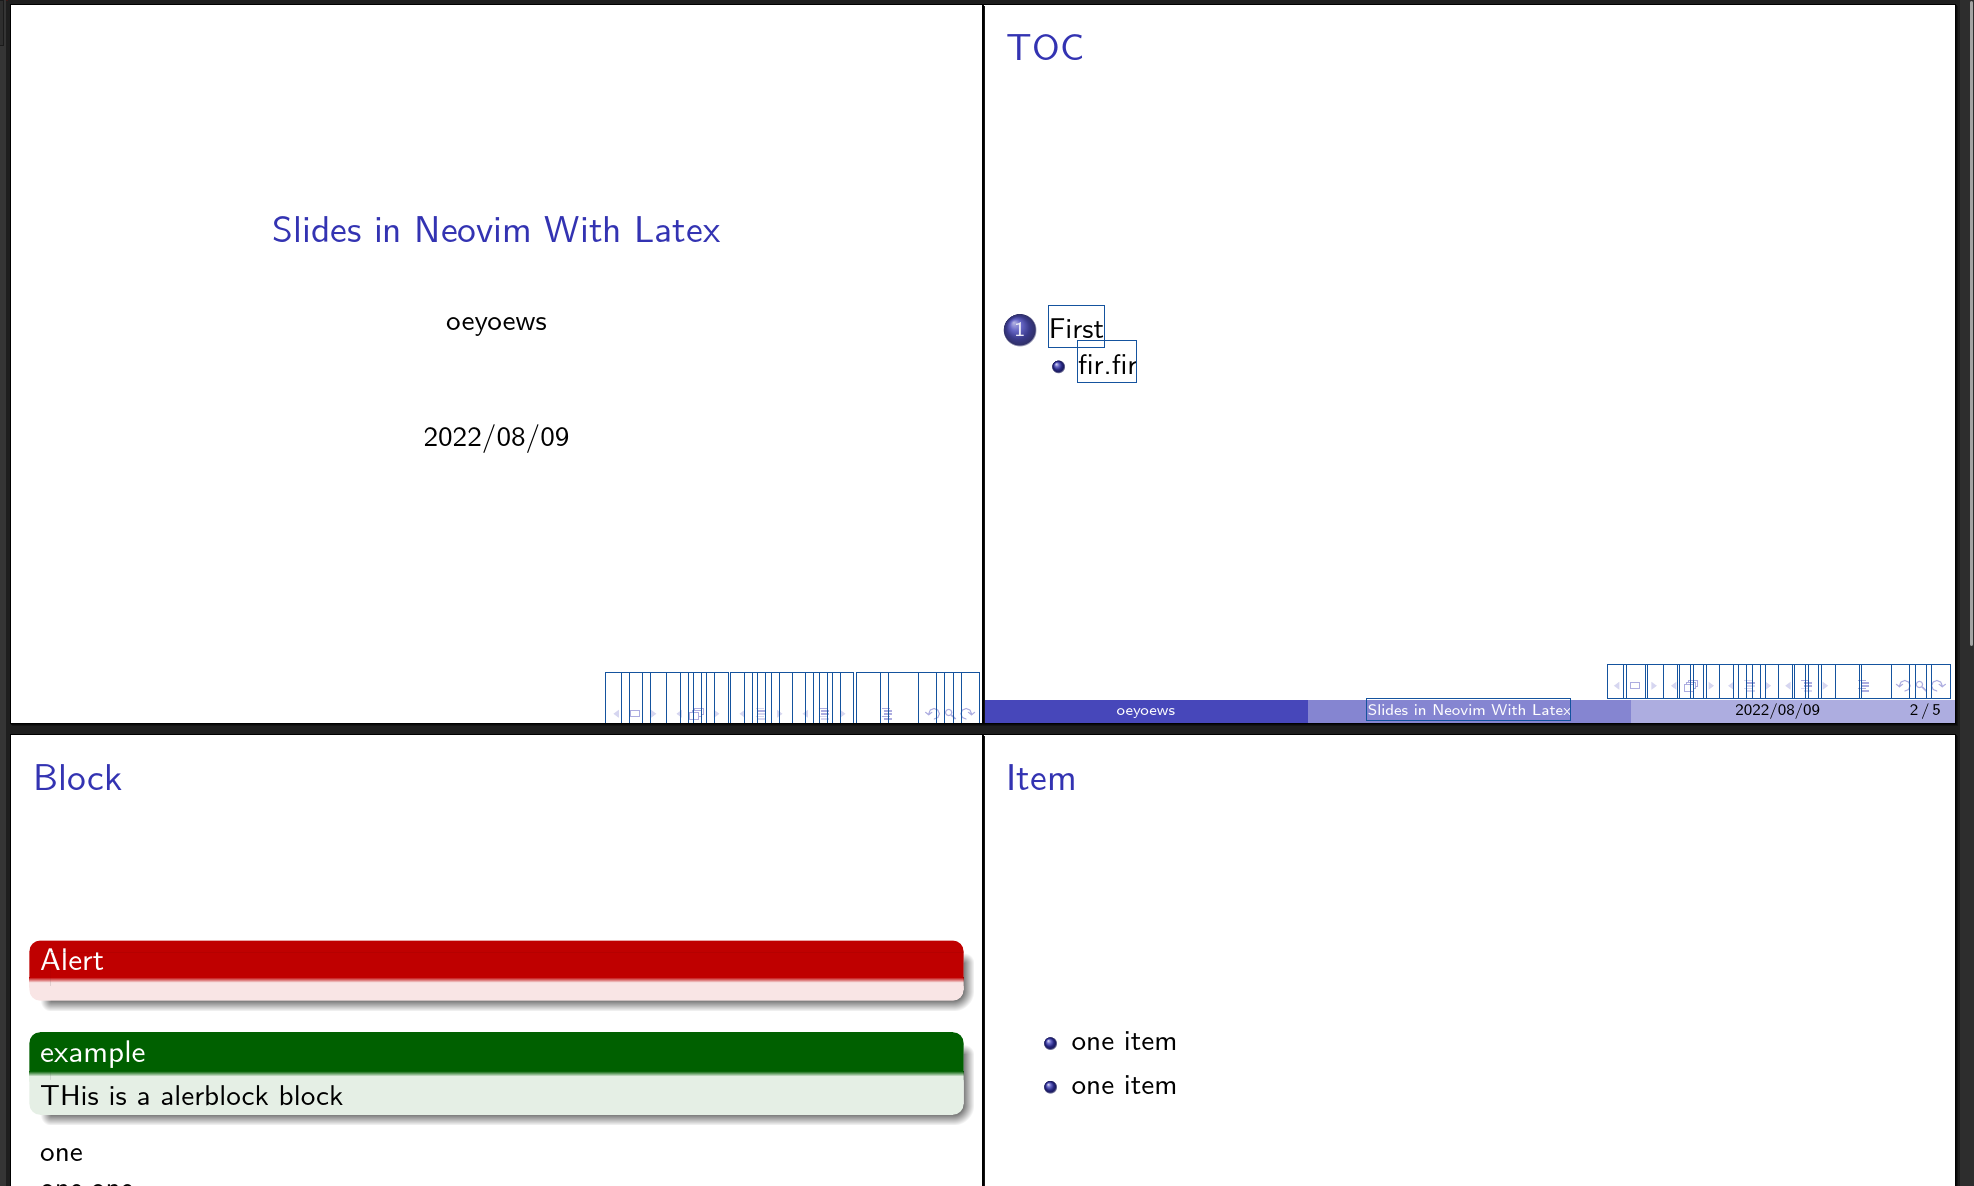
\includegraphics[width=0.7\textwidth]{img/01.png}
	\caption{Fig01}
	\label{Fig01}
	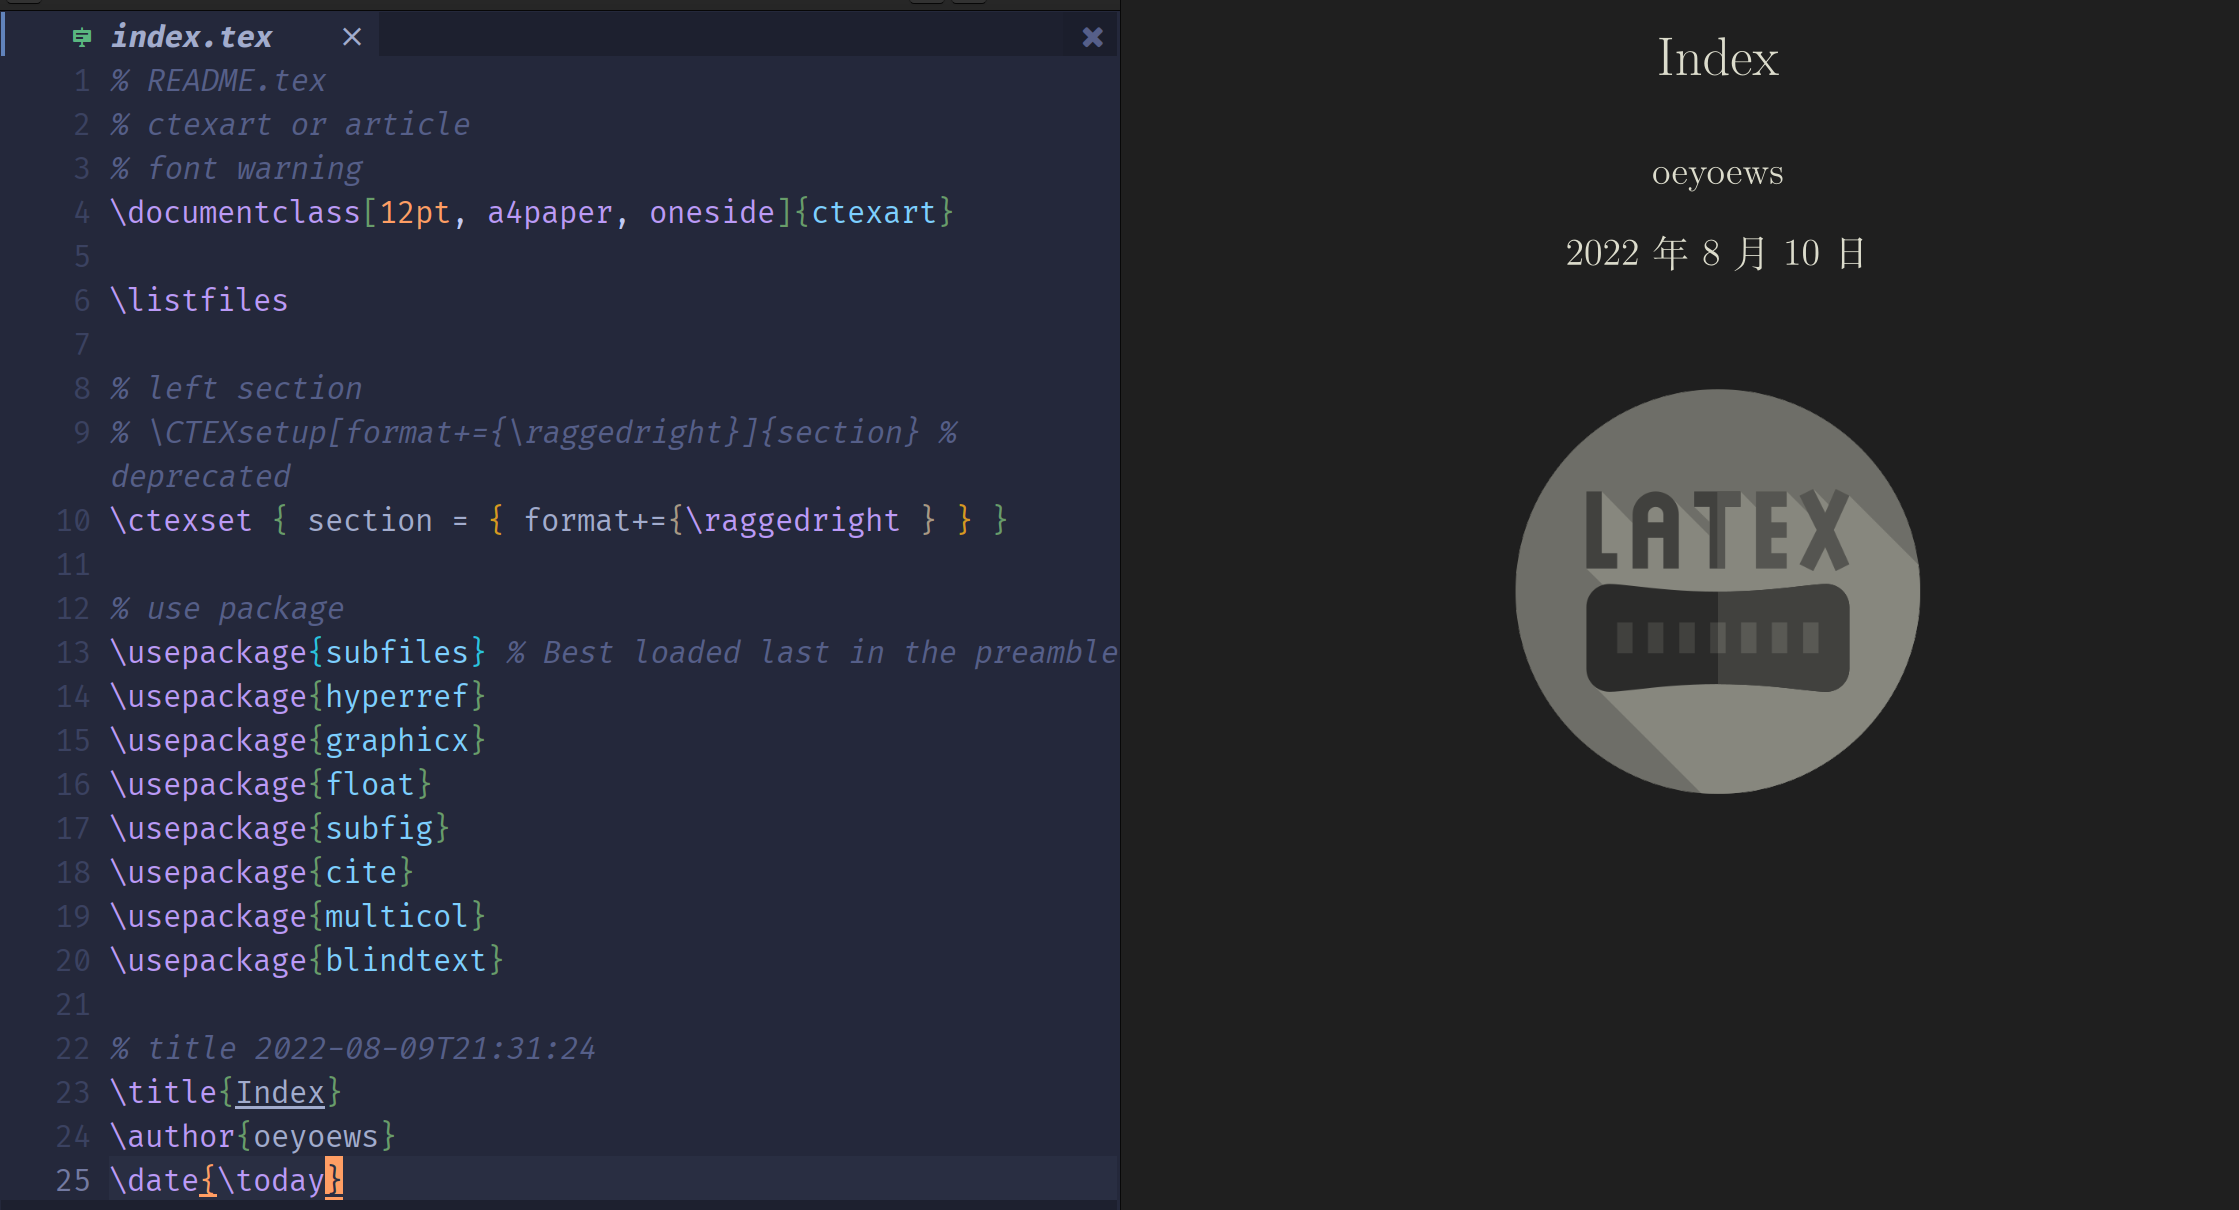
\includegraphics[width=0.7\textwidth]{img/02.png}
	\caption{Fig02}
	\label{Fig02}
\end{figure}

\end{document}

% paragraph.tex
\documentclass{ctexart}

\title{paragraph}
\author{oeyoews}
\date{2022/08/10}

\begin{document}

\maketitle

\section{Poetry}%
\label{sec:Paragraph}

% verse ??

% \centerline{ 蓦山溪·题钱氏溪月 }
%
% 与鸥为客,绿野留吟屐。两行柳垂阴,是当日、仙翁手植。一亭寂寞,烟外带愁横。荷苒苒,展凉云,横卧虹千尺。
%
% 才因老尽,秀句君休觅。万绿正迷人,更愁入、山阳夜笛。百年心事,惟有玉阑知,吟未了,放船回,月下空相忆。

\end{document}

% table.tex
\documentclass{article}

\usepackage{float}

\title{Table}
\author{oeyoews}
\date{2022/08/10}

\begin{document}

\maketitle

\section{Table}%
\label{sec:Table}

% https://evian-zhang.github.io/articles/LaTeX/LaTeX%E5%85%A5%E9%97%A8(%E4%B9%9D)/56495391.html
\begin{table}[H]
\centering
\caption{Title of table}
\begin{tabular}{|c|c|}\hline
a11&a12\\\hline
a21&a22\\\hline
\end{tabular}
\end{table}

\end{document}

\documentclass{article}

% https://blog.csdn.net/xovee/article/details/123087349
\usepackage{blindtext}
\usepackage{multicol}

\title{Multicols Demo}
\author{oeyoews}
\date{2022-08-10T12:23:42}

\begin{document}

\maketitle

\begin{multicols}{2}
[
\section{First Section}
All human things are subject to decay. And when fate summons, Monarchs must obey.
]
\blindtext\blindtext

This is second column
\end{multicols}

\end{document}

% test.tex
\documentclass[UTF8]{ctexart}

% Title left align
\ctexset { section = { format+={\raggedright } } }
\title{test}
\author{oeyoews}
\date{2022/08/11}

\begin{document}

\maketitle

% \tableofcontents
\section{Test include}%
\label{sec:Test include}

Hello, Latex use docmute test include
\end{document}

% forum.tex
\documentclass{article}

\usepackage{amsmath}

\title{Formula}
\author{oeyoews}
\date{2022/08/10}

\begin{document}

\maketitle

\section{Formula}%
\label{sec:Forum}

% example
\[
	\sqrt{x} + \sqrt{x^2} +\sqrt{y} = \sqrt[3]{k_i} - \frac{x}{m}
\]

% example
$$  \lim_{x \to \infty} x^2_{22} - \int_{1}^{5}x\mathrm{d}x + \sum_{n=1}^{20} n^{2} = \prod_{j=1}^{3} y_{j}  + \lim_{x \to -2} \frac{x-2}{x} $$

\subsection{inline formula}%
\label{sub:inline forum}

% example
$f = m^2$

\subsection{display block formula}%
\label{sub:display block forum}

% example
\[
	E = mc^2
	.\]

\subsection{Equation}%
\label{sec:equation}

\begin{align}
	f & = ma \\
	s & = vt
\end{align}

\begin{equation}
	A_{m,n} =
	\begin{pmatrix}
		a_{1,1} & a_{1,2} & \cdots & a_{1,n} \\
		a_{2,1} & a_{2,2} & \cdots & a_{2,n} \\
		\vdots  & \vdots  & \ddots & \vdots  \\
		a_{m,1} & a_{m,2} & \cdots & a_{m,n}
	\end{pmatrix}
\end{equation}

\subsection{Matrix}%
\label{sec:matrix}

% example
$$\begin{bmatrix}
		1      & 2      & \cdots \\
		67     & 95     & \cdots \\
		\vdots & \vdots & \ddots \\
	\end{bmatrix}$$

\subsection{math group}%
\label{sec:math}

\begin{equation}
	\left\{
	\begin{aligned}
		f = ma \\
		s = vt
	\end{aligned}
\right.
\end{equation}

\end{document}

\documentclass{article}

\usepackage{listings}
\usepackage{xcolor}

\lstset{numbers=left, %设置行号位置
        numberstyle=\tiny, %设置行号大小
        keywordstyle=\color{blue}, %设置关键字颜色
        commentstyle=\color[cmyk]{1,0,1,0}, %设置注释颜色
        frame=single, %设置边框格式
        escapeinside=``, %逃逸字符(1左面的键),用于显示中文
        %breaklines, %自动折行
        extendedchars=false, %解决代码跨页时,章节标题,页眉等汉字不显示的问题
        xleftmargin=2em,xrightmargin=2em, aboveskip=1em, %设置边距
        tabsize=4, %设置tab空格数
        showspaces=false %不显示空格
       }

\begin{document}

\section{CodeBlock}%
\label{sec:CodeBlock}

% \ lstinputlisting { source _ filename.py }

% not recongnize lua
\begin{lstlisting}[language=c]
printf("Lua code block")
\end{lstlisting}

\end{document}

%!TEX program = xelatex
% comment.tex
% \documentclass[UTF8]{ctexart}
\documentclass[UTF8]{article}

\usepackage{verbatim}
% Title left align
% \ctexset { section = { format+={\raggedright } } }
\title{comment}
\author{oeyoews}
\date{2022/08/11}

\begin{document}

\maketitle

\begin{comment}
 demo 
\end{comment}
% \tableofcontents

\section{comment} 
\end{document}

% tips.tex
\documentclass[UTF8]{article}

% Title left align
\title{tips}
\author{oeyoews}
\date{2022/08/11}

\begin{document}

\maketitle

\section{include}%
\label{sec:include}
Have import include includeonly, and subfile

\subsection{Term}%
\label{sec:term}
env, preamble, etc

\subsection{document}%
\label{sec:document}
gf to check source code , or check github one hundred tex files
\end{document}

%!TEX program = lualatex
% todo.tex
\documentclass[UTF8]{article}

\usepackage{emoji}

\title{todo \emoji{check-mark-button}}
\author{oeyoews}
\date{2022/08/11}

\begin{document}
% \setemojifont{TwemojiMozilla}

\maketitle

% \tableofcontents
\section{TODO \emoji{check-mark-button}}%
\label{sec:TODO}

\begin{itemize}
  \item img how to recursive search
  \item how use indenpend file, even have relative path, to compile
  \item this includeonly difference with include(linke cinclude and define? or
    input)
  \item solve relative path, such bib img
  \item this ref pag is not right
\end{itemize}
\end{document}

%!TEX program = xelatex
% hyper.tex
\documentclass[UTF8]{article}

\usepackage{showlabels}
% support cn, default is en
% \usepackage{ctex}

% Title left align
% \ctexset { section = { format+={\raggedright } } }
\title{hyper}
\author{oeyoews}
\date{2022/08/11}

\begin{document}

\maketitle

\section{hyperref}%
\label{sec:hyperref}
this is a hyper link

this \ref{sec:hyperref} is a dmeo
this \ref{sec:demo} si sec

\newpage

\section{demo}%
\label{sec:demo}

this second \pageref{sec:hyperref} demo

\end{document}

%!TEX program = xelatex
% compile.tex
\documentclass[UTF8]{article}

\usepackage{hyperref}
% support cn, default is en
% \usepackage{ctex}

% Title left align
% \ctexset { section = { format+={\raggedright } } }
\title{compile}
\author{oeyoews}
\date{2022/08/11}

\begin{document}

\maketitle

\section{hyper compile}%
\label{sec:hyper compile}

because the first time generate aux assist file, so this pdf will have question
symbol, in xelatex only one times.

but if use latexmk directly, this question will solved,(for two comile only
now), actually this command execute two time to generate pdf file, so it's
normal. \href{https://qa.1r1g.cn/tex/ask/17397131/}{latexmk virtue}

\end{document}


% ending
% ending.tex
\documentclass[UTF8]{ctexart}

\usepackage{graphicx}
\usepackage{float}
\usepackage{subfig}

\graphicspath{img/}

% Title left align
\ctexset { section = { format+={\raggedright } } }
\title{ending}
\author{oeyoews}
\date{2022/08/11}

\begin{document}

\maketitle

% \tableofcontents

\begin{figure}[htpb]
	\centering
	
\includegraphics[width=0.8\textwidth]{img/ending.png}
	\label{fig:img-ending-png}
\end{figure}

\end{document}


% special put reference site
\bibliographystyle{plain}
\bibliography{bib/all}

\end{document}
